% This is LLNCS.DEM the demonstration file of
% the LaTeX macro package from Springer-Verlag
% for Lecture Notes in Computer Science,
% version 2.4 for LaTeX2e as of 16. April 2010
%
\documentclass[citeauthoryear]{llncs}
%
%\usepackage{makeidx}  % allows for indexgeneration
%
\usepackage{algorithm,algorithmic}
\usepackage{multicol}
\usepackage{graphicx}           	% para manejar imagenes
\usepackage[utf8]{inputenc}

\begin{document}
\mainmatter              % start of the contributions
%
\title{Fast--BR and fast--CT\_EXT performance regarding basic matrix properties: an empirical study.}
%
\titlerunning{Fast--BR vs. CT_EXT}  % abbreviated title (for running head)
%                                     also used for the TOC unless
%                                     \toctitle is used
			 
\author{Vlad\'{i}mir Rodr\'{i}guez-Diez\inst{1,2} \and Jos\'{e}~Fco. Mart\'{i}nez-Trinidad\inst{1}
		 \and Jes\'{u}s~A. Carrasco-Ochoa\inst{1} \and Manuel~S.~Lazo-Cortés\inst{1}}
%
\authorrunning{Vlad\'{i}mir Rodr\'{i}guez et al.} % abbreviated author list (for running head)
%
%%%% list of authors for the TOC (use if author list has to be modified)
%\tocauthor{Ivar Ekeland, Roger Temam, Jeffrey Dean, David Grove,
%Craig Chambers, Kim B. Bruce, and Elisa Bertino}
%
\institute{Instituto Nacional de Astrof\'{i}sica, \'{O}ptica y Electr\'{o}nica,\\
		   Luis Enrique Erro \# 1, Tonantzintla, Puebla, M\'{e}xico,\\
		   Coordinaci\'{o}n de Ciencias Computacionales,\\
\email{vladimir.rodriguez@ccc.inaoep.mx}
\and Universidad de Camag\"{u}ey,\\
	 Circunvalaci\'{o}n Nte. km 5$\frac{1}{2}$, Camag\"{u}ey, Cuba}


\maketitle              % typeset the title of the contribution

\begin{abstract}
	Testor Theory is an important approach to feature selection in supervised classification. Typical testors are irreducible subsets of features preserving the object discernibility ability of the original set of features. 
%	A new dataset using only those features in a typical testor is a reduced representation of the original one, which improves the efficiency of machine learning tools without degrading their performance.
	Finding the complete set of typical testors for a dataset requires a high computational effort. Recent research has unveiled the relation of typical testors finding algorithms' performance with some properties of the basic matrix. In this paper, we make an empirical study involving two of the most recent and fastest algorithms of the state of the art: fast--BR and fast--CT\_EXT. Our study is carried out on synthetically generated basic matrices in order to control the properties under study.
%	, and results in a simple rule for selecting a priori the fastest algorithm for a given problem. Finally our empirical rule is evaluated on standard datasets.

\keywords{Testor Theory, Algorithms, Basic matrix properties}
\end{abstract}
%
\section{Introduction}
%
	Feature selection is an important task in supervised classification. It consists in identifying those features that provide relevant information for the classification process. This process may improve the efficiency of machine learning tools without degrading significantly their efficacy.
%	An information system is a dataset (table) containing objects (rows) which are	characterized by the value of some features (columns). A reduced representation of an information system, with the same discernibility between objects than that of the original dataset, reduces the computational	cost of the classification process. 
	In the Logical Combinatorial Pattern Recognition (Mart\'inez-Trinidad and Guzm\'an-Arenas~\cite{Martinez2001}), Testor Theory emerges as a solution to feature selection (Ruiz-Shulcloper~\cite{Shulcloper2008}). A testor is a subset of features which allows discerning between objects in different classes by using only its features. A Typical Testor (TT) is defined as a testor which is minimal with respect to inclusion. The main limitation to the application of the Testor Theory is that finding all the TTs has exponential complexity regarding the number of attributes in the dataset (Chikalov et al.~\cite{Chikalov13}).
	
	One of the first algorithms for finding all the TT, called BT (Ruiz-Shulcloper et al.~\cite{Shulcloper1982}), codified a subset of features as a binary word with as many bits as features in the dataset. A 0 represents the absence of the corresponding feature in the current	subset while a 1 represents its inclusion. In this way, candidate subsets are evaluated in the natural order of binary numbers. The pruning process in the	search space is based on the minimal condition of TT and a convenient sorting of the basic matrix associated to the dataset. In (Ruiz-Shulcloper et al.~\cite{Shulcloper1995b}) a new algorithm (REC) is presented.	The main drawback of REC is that it operates directly over the dataset (instead of the	basic matrix), handling a huge amount of superfluous information. Ayaquica~(\cite{Ayaquica1997})	presented the algorithm CER directed to solve this problem by using a different traversing	order. 
	
	Then, Santiesteban and Pons-Porrata~(\cite{Santiesteban2003}) proposed a new algorithm called LEX. The main ideas behind LEX are a new traversing order of candidates (which resembles the	lexicographical order in which string characters are compared) and the concept of gap. In LEX the typical condition is verified first and only for those potentially TTs, the testor condition is checked. This way, the out-coming testors from this algorithm are always typical. Once obtained a TT (or a not testor) candidate which includes the last feature in the dataset, the concept of gap allows us avoiding any subset of this candidate.
	
	Sanchez-D\'iaz and Lazo-Cort\'es~(\cite{Sanchez2007}) proposed the CT\_EXT algorithm for computing all TT. Following a traversing order similar to that in LEX, this algorithm searches for testors without verifying the typical condition. In this way, a larger number of candidates is usually evaluated, in comparison to LEX; but the cost of each evaluation is lower. The authors show that CT\_EXT is faster than the previous existing algorithm for most datasets. Then, Lias-Rodr\'iguez and Pons-Porrata~(\cite{Lias2009}) presented the BR algorithm, a Recursive algorithm based on Binary operations. BR is similar to LEX in its bones but its recursive nature encloses a reduction in the number of evaluated candidates. Given a candidate subset, the remaining features are tested a priori and those being rejected are excluded from subsequent evaluations. Sanchez-D\'iaz et al.~(\cite{Sanchez2010}) presented a cumulative procedure for the CT\_EXT algorithm. This fast-CT\_EXT implementation drastically reduces the runtime for most datasets at no extra cost. In (Lias-Rodr\'iguez and Sanchez-D\'iaz~\cite{Lias2013}) the gap elimination and column reduction are added to BR. The main drawback of fast-BR and BR is, as in LEX, the high cost of evaluating the typical condition for every contributing candidate. 
	
	We have described above the evolution of the so called \emph{external scale} algorithms for typical testor computation. In addition, a different line of algorithms such as CT (Bravo-Martínez~\cite{Bravo83}), CC (Águila and Ruíz-Shulcloper~\cite{Aguila84}) and YYC (Alba-Cabrera et al.~\cite{Alba14}) has been developed. These kind of algorithms are called \emph{internal scale} algorithms, and they analyze the basic matrix to find out some conditions to guarantee that a subset of attributes is a typical testor. Internal scale algorithms usually evaluate less candidates than external scale algorithms but each candidate evaluation has a higher computational cost. Therefore, the search for fast algorithms for computing typical testors has been biased to external scale algorithms (Alba-Cabrera et al.~\cite{Alba14}).
	
	Recently, a thorough study presented in (Alba-Cabrera et al.~\cite{Alba13}) concluded that no single typical testor finding algorithm have the best performance for any given problem. Other studies (Lias-Rodr\'iguez and Sanchez-D\'iaz~\cite{Lias2013}, Rodríguez-Diez et al.~\cite{Rodriguez15}), categorize basic matrices by the density of 1's they have; i.e. the number of ones divided by the total number of cells of the matrix. Furthermore, González-Guevara et al.~(\cite{Gonzalez15}) referred a series of elements that influence the algorithms' performance, such as the number of rows, the density of 1's and the number of typical testors of the basic matrix. With these precedents, in this paper we present an empirical study to identify a relationship between some of these properties of the basic matrix and the performance of the most successful algorithms:  fast--CT\_EXT (Sanchez-D\'iaz et al.~\cite{Sanchez2010}) and fast--BR (Lias-Rodr\'iguez and Sanchez-D\'iaz~\cite{Lias2013}). From this empirical study we obtained a simple rule to determine a priory the fastest algorithm for a determined dataset. Finally we evaluated our rule on standard datasets from the UCI dataset repository (Bache and Lichman~\cite{Bache13}). 
	
%
\section{Basic Concepts}
%
	In this section, we introduce the main concepts, definitions and propositions supporting the pruning strategies of fast--CT\_EXT and fast--BR. Here, we aim to provide the key elements to understand the differences between these two algorithms. 
	
	Let $DS$ be a dataset with $k$ objects described by $n$ attributes (features) and grouped in $r$ classes. Every attribute in the set of attributes $R=\lbrace x_1,...,x_n \rbrace$, may be of any type and has predefined a comparison criterion (usually the simple equality). Let $DM$ be the binary comparison matrix obtained from comparing every pair of objects in $DS$ belonging to different classes. Every comparison of a pair of objects adds a row to $DM$ with 0=equal,1=different in the corresponding attribute position (column). $DM$ has $m$ rows and $n$ columns. Comparisons generating a row with only 0's, hereinafter referred to as empty row, imply that two objects from different classes are equal by their attributes values. 
	%These rows are called inconsistencies of $DS$ and are not included in $DM$.
	
	\begin{definition}\label{def:testor}
		Let $T \subseteq R$ be a subset of attributes from $DS$. We say that T is a testor if in the sub-matrix
		of DM formed by the columns corresponding to attributes in T, there is not any empty row.
	\end{definition}
	
%	An empty row in this sub-matrix of $DM$ imply that the reduced dataset obtained from $DS$, using only those attributes in $T$, has more equal objects in different classes than $DS$. 	
	
	Usually the number of rows in $DM$ ($m$) is large. Lazo-Cort\'es et al.~(\cite{Lazo2001}) proposed a reduction of $DM$ without loosing relevant information. They proved that this reduced matrix, called \textit{basic matrix} ($BM$), and $DM$; have the same set of testors. Then, we can substitute $DM$ by $BM$ in the definition~\ref{def:testor} without any loose of generality. 
	
%	\begin{definition} \label{def:BM}
%		Let $S_{j} \subseteq R$ be a subset of attributes associated to the row j of DM, such that $x_i \in S_{j}$ iff the row j has a 1 in the column i. And let $SS=\lbrace S_1, S_2,...,S_m  \rbrace$ be the set of possible subsets $S_{j}$ in DM. The Basic Matrix BM of DS is formed by all the rows in DM (without repetitions) for which its associated $S_{j}$ has not any proper subset in SS.
%	\end{definition}	
	
	
	\begin{definition}\label{def:TT}
		A subset of attributes $T \subseteq R$ is a typical testor in BM iff T is a testor and $\forall x_i \in T, T \setminus x_i$ is not a testor. 
	\end{definition}
		
%	
\subsection{Concepts for fast--CT\_EXT}
%
		
	\begin{definition}\label{def:contrib}
		Given $T \subseteq R$ and $x_i \in R$ such that $x_i \notin T$. We say that $x_i$ contributes to T iff the sub-matrix of BM formed with only those attributes in T has more empty rows than that formed with attributes in $T \cup \lbrace x_i \rbrace$.
	\end{definition}	
	
	The core of the CT\_EXT algorithm is supported by propositions~\ref{prop:contrib} and~\ref{prop:superset}; which are stated and proved in (Sanchez-D\'iaz et al.~\cite{Sanchez2010}) (Theorems 1 and 2 respectively).
	
	\begin{proposition}\label{prop:contrib} 
		Given $T \subseteq R$ and  $x_i \in R$ such that $x_i \notin T$. If $x_i$ does not contribute to T, then 		$T\cup\{x_i\}$ cannot be a subset of any typical testor.
	\end{proposition}

	\begin{proposition}\label{prop:superset} 
		Given $T \subseteq R$ and $Z \subseteq R$ such that $Z \cap T = \emptyset$. If T is a testor, then $T \cup Z$ is a 	testor too, but it is not a typical testor.
	\end{proposition}

%
\subsection{Concepts for fast--BR}
%
	In addition to the propositions exposed above, fast--BR is supported by the following propositions; which are stated and proved in (Lias-Rodr\'iguez and Sanchez-D\'iaz~\cite{Lias2013}).

%	\begin{proposition}\label{prop:recursive} 
%		Given $T \subseteq R$, $Z \subseteq R$ and  $x_i \in R$ such that $x_i \notin Z$ and $T \subseteq Z$. If $x_i$ does not contribute to T or form a testor with T, then $Z\cup\{x_i\}$ cannot be a subset of any typical testor.
%	\end{proposition}	
%	
%	Proposition~\ref{prop:recursive} constitutes the basis for the recursive implementation of the algorithm. Fast--BR introduces a kind of look ahead variant to the lexicographical order to take advantage of this proposition. This procedure avoids subsequent evaluations of a non contributing attribute.
	
	\begin{definition}\label{def:exclusion}
		Given $T \subseteq R$ we call compatibility mask of $T$, denoted as $cm_T$, to the binary word in which the $j^{\mathit{th}}$ bit is 1 if the $j^{\mathit{th}}$ row of $BM$ has a 1 in only one of the columns corresponding to attributes in $T$, and otherwise it is 0.
	\end{definition}
	
	\begin{proposition}\label{prop:exclude} 
		Given $T \subseteq R$ and $x_i \in R$ such that $x_i \notin T$.	We denote $c_{x_k}$ to the binary word in which the $j^{\mathit{th}}$ bit is 1 if the $j^{\mathit{th}}$ row of $BM$ has a 1 in the column corresponding to $x_k$. If $\exists x_k \in T$ such that $cm_{T \cup \lbrace x_i\rbrace} \wedge c_{x_k}=(0,...,0)$. Then, $T \cup \lbrace x_i\rbrace$ cannot be a subset of any typical testor. And we will say that $x_i$ is exclusionary with $T$.
	\end{proposition}
	
	We will refer to Proposition~\ref{prop:exclude} as exclusion evaluation. The application of the exclusion evaluation for typical testor property identification is given in the form of Proposition~\ref{prop:TT}.
	
	\begin{proposition}\label{prop:TT} 
			Given $T \subseteq R$ and $x_i \in R$ such that $x_i \notin T$. The subset $T \cup \lbrace x_i\rbrace$ is a typical testor iff it is a testor and $x_i$ is not exclusionary with $T$.
	\end{proposition}
		
%
\section{Comparative Study}
%
	  From our literature review, we found two families of external scale algorithms: those evaluating first the testor condition and then verifying the typical condition (exclusion evaluation), and those evaluating the exclusion first and then the testor condition. We include in our comparative study the main exponents of these two families: fast--CT\_EXT and fast--BR, respectively. Their candidate evaluation process is illustrated in Figure~\ref{fig:candeval}.  Since the number of testors is usually a small fraction of the total evaluated candidates, we can state that most of the times fast--BR makes more exclusion evaluations than fast--CT\_EXT. For our experimental study in the next section we will use the algorithms implementations provided by their authors\footnote{The source code as well as all the basic matrices and datasets used in our experiments can be downloaded from \url{http://ccc.inaoep.mx/$\sim$ariel/CTBRES}}.

	\begin{figure}[htb]
	    \centering
	    \begin{minipage}{.5\textwidth}
	        \centering
	        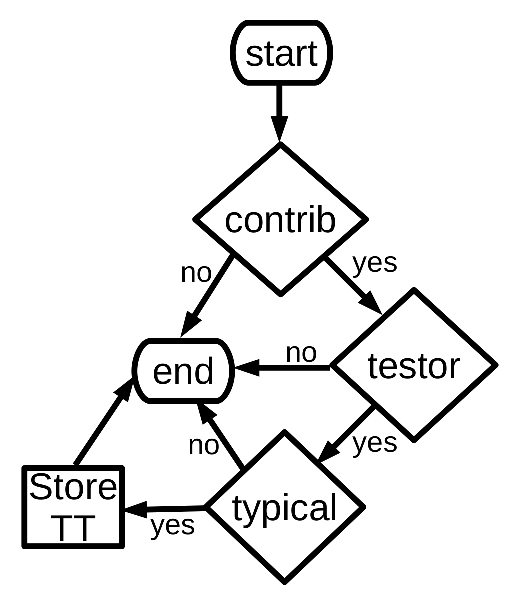
\includegraphics[height=4cm]{ct_ext.eps}
	    \end{minipage}%
	    \begin{minipage}{0.5\textwidth}
	        \centering
	        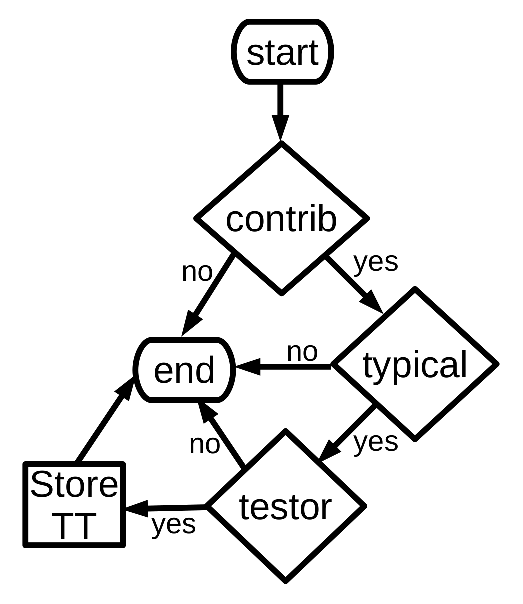
\includegraphics[height=4cm]{BR.eps}	        
	    \end{minipage}
		\caption{Candidate evaluation flowchart for fast--CT\_EXT (left) and fast--BR (right).}
		\label{fig:candeval}
	\end{figure}
	
%
\subsection{Comparison over synthetic basic matrices}
%
In order to explore the influence of the basic matrix density on the relative performance of fast--CT\_EXT and fast--BR; we conducted this first experiment over 500 randomly generated basic matrices with 2000 rows and 30 columns. The size of these matrices was selected in order to keep reasonable runtime for the three algorithms. Our 500 matrices were generated with densities of 1's uniformly distributed in the range (0.16--0.80) using a step of 0.04. 

	\begin{figure}[htb]
	    \centering
	    \begin{minipage}[b]{0.48\textwidth}
	        \centering
	        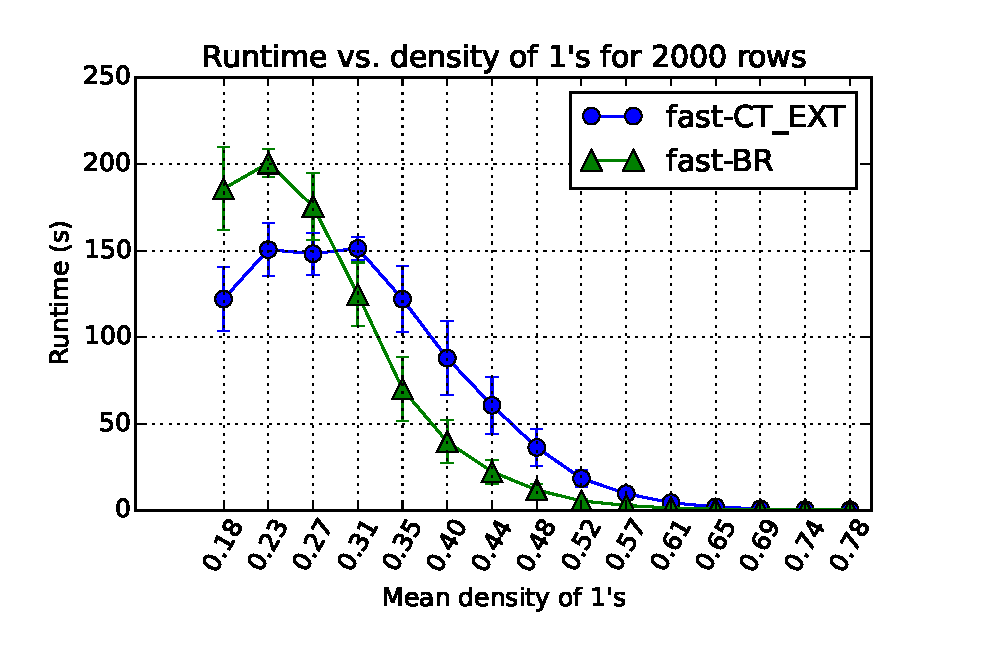
\includegraphics[height=4cm]{2000rows.eps}	        
	        \caption{Runtime vs. density for basic matrices with 2000 rows.}
	        \label{fig:density}
	    \end{minipage}
	    \begin{minipage}[b]{0.48\textwidth}
	    	\centering
	    	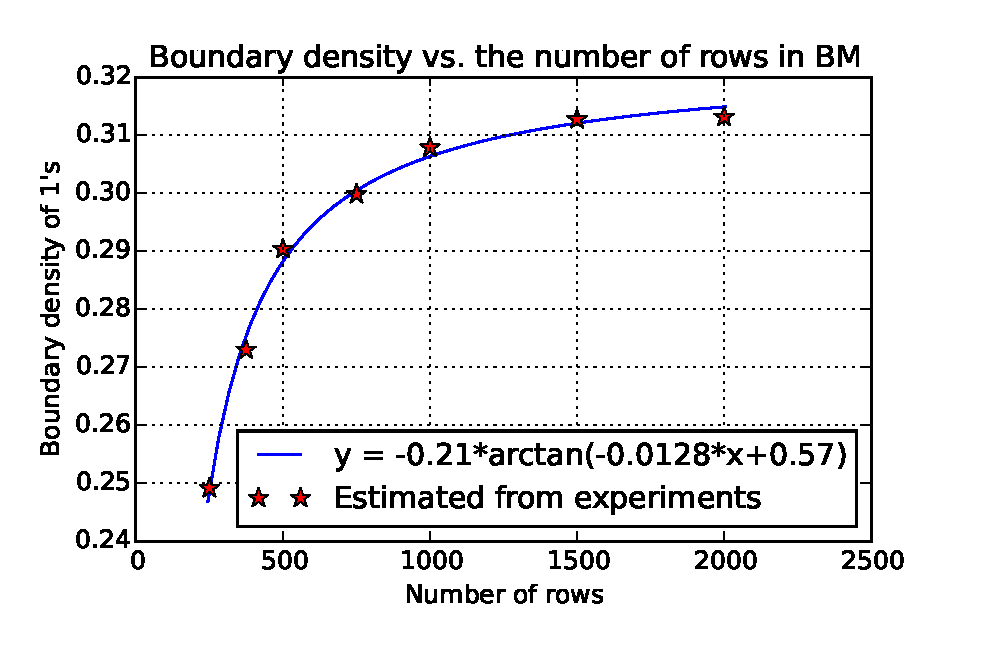
\includegraphics[height=4cm]{fitting.eps}	        
	    	\caption{Boundary density regarding the number of rows in BM.}
	    	\label{fig:fitting}
	    \end{minipage}
	\end{figure}

	From Fig.~\ref{fig:density}, it can be seen that fast--CT\_EXT was faster for basic matrices with density under 0.31, while fast--BR was faster for matrices with density above 0.31. To understand this behavior, we must look back to Fig.~\ref{fig:candeval}. The exclusion evaluation has the higher computational complexity in both algorithms ($\Theta (nm)$). Exclusionary attributes are found when there is at least one column in the basic matrix, considering only those attributes in the current candidate, that can be removed without increasing the number of zero rows. This condition is more frequent in matrices with higher density, where overlapping of 1's is most likely. For matrices with a relative high density, the heavier candidate evaluation process of fast--BR pays off, because exclusionary attributes are avoided from subsequent evaluations. For matrices with lower density, the simpler approach of fast--CT\_EXT results in a faster execution. Take for instance the extreme case of the identity matrix, where there is not any exclusionary attribute, since they are all indispensable to form a typical testor. For this kind of basic matrices, fast--CT\_EXT needs to evaluate as many candidates as fast--BR but the former makes a single exclusion evaluation with the set of all attributes. On the other hand, fast--BR evaluates the exclusion for each candidate, which leads to a higher computational cost.
	
	In order to evaluate the influence of the number of rows in the basic matrix over the relative performance of the two algorithms, we repeated this first experiment for matrices with different number of rows. Each time, 500 basic matrices with the same number of rows and 30 columns was generated following a density distribution similar to that of our first experiment. The number of rows and the obtained density boundary for each experiment are shown in Fig.~\ref{fig:fitting}. The boundary density for each point was estimated by fitting the runtime for each algorithm by a third degree polynomial and finding their interception. The continuous line in Fig.~\ref{fig:fitting} corresponds to a least-squares fitting. We used an arctangent function to model the apparent saturation of the boundary density ($d_\beta$) with the increase of the number of rows ($m$), as suggested in (Durmiak~\cite{Durmiak}). In addition, we found that for matrices with 125 rows fast--BR was always faster. We can say then, that for those datasets which have a basic matrix with a density of ones lower than $d_\beta=-0.21\tan^{-1}(-0.0128m+0.57)$ which have $m\geq250$, fast--CT\_EXT is faster and otherwise fast--BR is faster. For values close to this boundary, the rule should be interpreted carefully due to the random behavior of these algorithms. What we can expect from these basic matrices, with a density close to the boundary, is an insignificant runtime difference between the two algorithms, as it can be seen in Fig.~\ref{fig:density}.
%
\subsection{Evaluation on standard datasets}
	In order to evaluate the rule obtained from synthetic basic matrices, we selected 10 datasets from the UCI database repository (Bache and Lichman~\cite{Bache13}). Table~\ref{tab:density} shows the runtime for fast--CText and fast--BR over our selected datasets.
	
	\begin{table}[htb]
		\centering \footnotesize
		\caption{Fast--CText and fast--BR runtimes for standard datasets. Sorted by basic matrix density.}
		\label{tab:density}
		\begin{tabular}{lcccccrr}
			\hline
			&&&& \multicolumn{2}{c}{Basic Matrix} &  \multicolumn{1}{c}{Fast--CText} & \multicolumn{1}{c}{Fast--BR} \\
			\cline{5-6}
			Dataset   		 & Attributes & Instances & TTs     & rows  & density & runtime (s) & runtime (s) \\
			\hline
			Keyword-activity & 37         & 1530      & 3        & 26    & 0.04    & 1.22             & \textbf{0.90}   \\
			Connect-4        & 43         & 6756      & 35       & 406   & 0.05    & 12876.67         & \textbf{160.61} \\
			QSAR-biodeg      & 42         & 1055      & 256      & 40    & 0.12    & 0.75             & \textbf{0.33}   \\
			Credit-g         & 21         & 1000      & 846      & 223   & 0.35    & \textbf{0.05}    & 0.12            \\
			Flags            & 30         & 194       & 23543    & 390   & 0.35    & \textbf{1.00}    & 1.06            \\
			Student-por      & 32         & 649       & 851584   & 8158  & 0.41    & 1874.57          & \textbf{161.35} \\
			Sponge           & 46         & 76        & 10992    & 68    & 0.42    & 0.63             & \textbf{0.14}   \\
			Student-mat      & 32         & 395       & 679121   & 6904  & 0.43    & 1003.87          & \textbf{81.82}  \\
			Lung-cancer      & 57         & 32        & 4183355  & 237   & 0.47    & 188.20           & \textbf{7.34}   \\
			Cylinder-bands   & 40         & 512       & 23534    & 1147  & 0.55    & 5.03             & \textbf{0.53}   \\
			\hline
		\end{tabular}
	\end{table}
	
 Notice that according to our previous study, the only dataset for which fast--CText should be clearly faster is Connect-4. Nevertheless, fast--BR was two orders of magnitude faster for this dataset. This can be explained because the basic matrix associated to this dataset has several null and duplicated columns. Fast--BR takes advantage of this issue (which is not present in our synthetic matrices) by means of the column reduction (Lias-Rodr\'iguez and Sanchez-D\'iaz~\cite{Lias2013}) and avoids a huge amount of meaningless candidate verifications. We believe, however, that this capability can be easily introduced into fast--CText without modifying the algorithm essence. For Credit-g and Flags datasets, fast--CText was faster but the runtime difference is insignificant because their basic matrices have densities close to our predicted boundary.
 
%
\section{Conclusions}
%
 This paper presents an empirical study on the relation of two typical testors finding algorithm's performance with some properties of the basic matrices. We selected for this study the main exponents of the two ways of doing of external scale algorithms: fast--CText and fast--BR. A set of synthetically generated matrices were used to explore their performance regarding the density of 1's and the number of row of the basic matrix. From our experimental results, we obtained a simple rule for selecting a priori the fastest algorithm for a given dataset. We think; however, that the main contribution of this paper is the introduction of a new approach to the assessment of typical testors finding algorithm's performance. This approach provides more substantial information than the traditional evaluation over a random sample of datasets.
 
 The evaluation over standard datasets from the UCI database repository, reflected the advantages of the column reduction process included in fast--BR. Thus, future work can be directed to introduce this capability into fast--CT\_EXT. Furthermore, the relation of algorithm's performance with the number of columns in the basic matrix should be also studied.

% ---- Bibliography ----
%
\begin{thebibliography}{}
%
% TODO poner los títulos en inglés

\bibitem[1984]{Aguila84}	
	Águila, L., Ruíz-Shulcloper, J.  
	Algorithm CC for the elaboration of k-valued information on pattern recognition problems. 
	Mathematics Sciences Journal (In Spanish), 
	5(3) (1984)
	
\bibitem[2013]{Alba13}
	Alba-Cabrera, E., Ibarra-Fiallo, J.,Godoy-Calderon, S.:
	A Theoretical and Practical Framework for Assessing the Computational Behavior of Typical Testor-Finding Algorithms.
	In CIARP 2013, Part I. LNCS,
	8258, 351--358, (2013)
	
\bibitem[2014]{Alba14}
	Alba-Cabrera, E., Ibarra-Fiallo, J., Godoy-Calderon, S., Cervantes-Alonso, F.:
	YYC: A Fast Performance Incremental Algorithm for Finding Typical Testors.
	Progress in Pattern Recognition, Image Analysis, Computer Vision, and Applications.
	416--423 (2014)
	
\bibitem[1997]{Ayaquica1997}
	Ayaquica, I. O.:
	A new external scale algorithm for typical testor computation.
	Memories of the Second International Workshop on Pattern Recognition (In Spanish), 
	Havana, 141--148 (1997)
	
\bibitem[2013]{Bache13}	
	Bache, K., Lichman, M.:
	UCI machine learning repository.
	(2013)
	
\bibitem[1983]{Bravo83}	
	Bravo-Martínez, A.:
	Algorithm CT for Calculating the Typical Testors of k-valued Matrix. 
	Mathematics Sciences Journal (In Spanish), 
	4(2), 123--144 (1983)
	
\bibitem[2013]{Chikalov13}	
	Chikalov, I., Lozin, V. V., Lozina, I., Moshkov, M., Nguyen, H. S., Slowron, A., Zielosko, B.:
 	Three approaches to data analysis. 
 	Springer Science \& Business Media, 
 	(2013)
	
\bibitem[2000]{Durmiak}	
	Durmiak, A.:
	Fitting saturation and hysteresis via arctangent functions. 
	IEEE Power Engineering Review,
	20(11), 55--57 (2000)

\bibitem[2015]{Gonzalez15}		
	González-Guevara, V., Godoy-Calderón, S., Alba-Cabrera, E.,  Ibarra-Fiallo, J.:
	A Mixed Learning Strategy for Finding Typical Testors in Large Datasets. 
	In CIARP 2015. LNCS,
	5197, 716--723 (2008)
		
\bibitem[2001]{Lazo2001}	
	Lazo-Cort\'es, M., Ruíz-Shulcloper, J., Alba-Cabrera, E.:
	An Overview of the Evolution of the Concept of Testor. 
	Pattern Recognition. 34, 753--762 (2001)

\bibitem[2009]{Lias2009}
	Lias-Rodr\'iguez, A., Pons-Porrata, A.:
	BR: A new method for computing all typical testors. 
	Lecture Notes in Computer Science.
	5856 LNCS, 433--440 (2009)

\bibitem[2013]{Lias2013}	
	Lias-Rodr\'iguez, A., Sanchez-D\'iaz, G.:
 	An Algorithm for Computing Typical Testors Based on Elimination of Gaps and Reduction of Columns.
 	International Journal of Pattern Recognition and Artificial Intelligence. 27(08), 1350022 (2013)

\bibitem[2001]{Martinez2001}
	Mart\'inez-Trinidad, J.F., Guzm\'an-Arenas, A.: 
	The Logical Combinatorial Approach to Pattern Recognition an Overview through Selected Works. 
	Pattern Recognition. 34, 741--751 (2001)

\bibitem[2015]{Rodriguez15}	
	Rodríguez-Diez, V., Martínez-Trinidad, J. F., Carrasco-Ochoa, J. A., Lazo-Cortés, M., Feregrino-Uribe, C., Cumplido, R.:
	A fast hardware software platform for computing irreducible testors. 
	Expert Systems with Applications, 
	42(24), 9612–9619 (2015)

\bibitem[1995b]{Shulcloper1995b}
	Ruíz-Shulcloper, J., Alba-Cabrera, E., Lazo-Cort\'es, M.:
	Introduction to Typical Testors theory.
	Green Series (In Spanish), No. 50 . CINVESTAV-IPN, México, (1995)
	
\bibitem[1982]{Shulcloper1982}	
	Ruíz-Shulcloper, J., Aguila, L., Bravo, A.:
	BT and TB algorithms for computing all irreducible testors. 
	Mathematics Sciences Journal (In Spanish), 2, 11--18 (1982)

\bibitem[2008]{Shulcloper2008}
	Ruíz-Shulcloper, J.:
	Pattern recognition with mixed and incomplete data. 
	Pattern Recognition and Image Analysis. 18(4), 563--576 (2008)
	
\bibitem[2007]{Sanchez2007}
	Sanchez-D\'iaz, G., Lazo-Cort\'es, M.:
	CT-EXT: an algorithm for computing typical testor set. 
	In Progress in Pattern Recognition, Image Analysis and Applications. 
	Springer. 506--514 (2007)

\bibitem[2010]{Sanchez2010}
	Sanchez-D\'iaz, G., Piza-Davila, I., Lazo-Cort\'es, M., Mora-Gonz\'alez, M., Salinas-Luna, J.:
	A fast implementation of the CT-EXT algorithm for the testor property identification. 
	Lecture Notes in Computer Science, 6438 LNAI(PART 2), 92--103 (2010)

\bibitem[2003]{Santiesteban2003}	
	Santiesteban, Y., Pons-Porrata, A.:
	LEX: a new algorithm for the calculus of typical testors. 
	Mathematics Sciences Journal (In Spanish), 21(1), 85--95 (2003)
	
	
\end{thebibliography}

%\clearpage
%\addtocmark[2]{Author Index} % additional numbered TOC entry
%\renewcommand{\indexname}{Author Index}
%\printindex
%\clearpage
%\addtocmark[2]{Subject Index} % additional numbered TOC entry
%\markboth{Subject Index}{Subject Index}
%\renewcommand{\indexname}{Subject Index}
%\input{subjidx.ind}
\end{document}
